For donwloads of:
\begin{itemize}
	
\item pointing models, contact OOD,
\item delay models, contact AOD 
\item receiver models, see procedure below.
\end{itemize}
\section{ Receiver Models Updates}
\begin{itemize}
	

\item[\textbf{Step 1}] Whenever a receiver is replaced on a receptor, check the '\sensor{rsc.rx?.rec-model-date}' sensor (where \sensor{?} is the band) of that receptor. Compare the value you found with the value given in the table found in this document. If there is a difference, the receiver models need to be updated and thus proceed to step 2 If the values are the same, no action is required.


\begin{figure}[!thb]
	\centering
	%\includegraphicsdpi{100}{}{bur1.png}     
	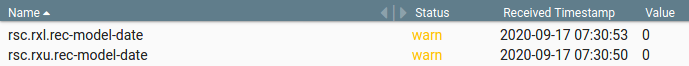
\includegraphics[scale=0.5]{Chapters/images/image77.png}
	
	%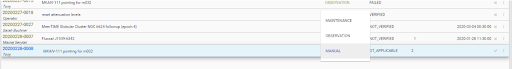
\includegraphics[resolution=100]{bur1.png}
	\caption{Receiver model date sensors}
	\label{fig:image77}
\end{figure}

\item[\textbf{Step 2}] A script is in place to download and push the models to GitHub. Do the following:
\begin{lstlisting}[style=DOS]
$ ssh user@mkat-thn-linux.mkat.karoo.kat.ac.za 

\end{lstlisting}

	

\item Here “user” refers to your FreeIPA username (the one you use to log in to sites like EduVPN and Mattermost). When it asks you for a password, use your FreeIPA password.
\begin{lstlisting}[style=DOS]
$ cd ../msteyn/download\_rx\_models
$ ./run\_rx\_models_download.sh --ant m0xx --band (l or u)

\end{lstlisting}


\item This will output an instruction with receiver serial number. Copy or add the serial number as the second argument.


\begin{figure}[!thb]
	\centering
	%\includegraphicsdpi{100}{}{bur1.png}     
	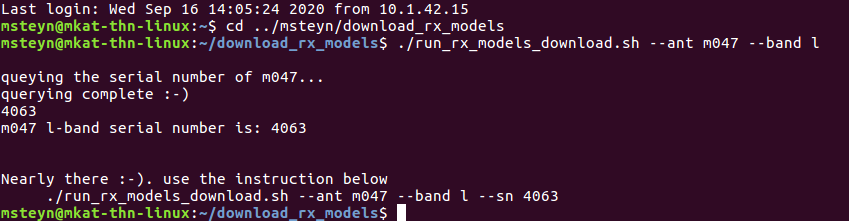
\includegraphics[scale=0.5]{Chapters/images/image89.png}
	
	%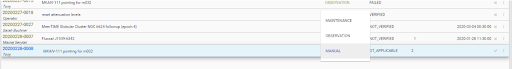
\includegraphics[resolution=100]{bur1.png}
	\caption{Receiver model downloads}
	\label{fig:image89}
\end{figure}

\begin{lstlisting}[style=DOS]
$ ./run_rx_models_download.sh --ant m0xx --band (l or u) --sn xxxx

\end{lstlisting}


\item At some point the script will prompt you to enter your FreeIPA username (it’s the one you use to log in to sites like EduVPN and Mattermost).



\item When prompted enter “rsc” as the password to download the models to your local directory.

\begin{figure}[!thb]
	\centering
	%\includegraphicsdpi{100}{}{bur1.png}     
	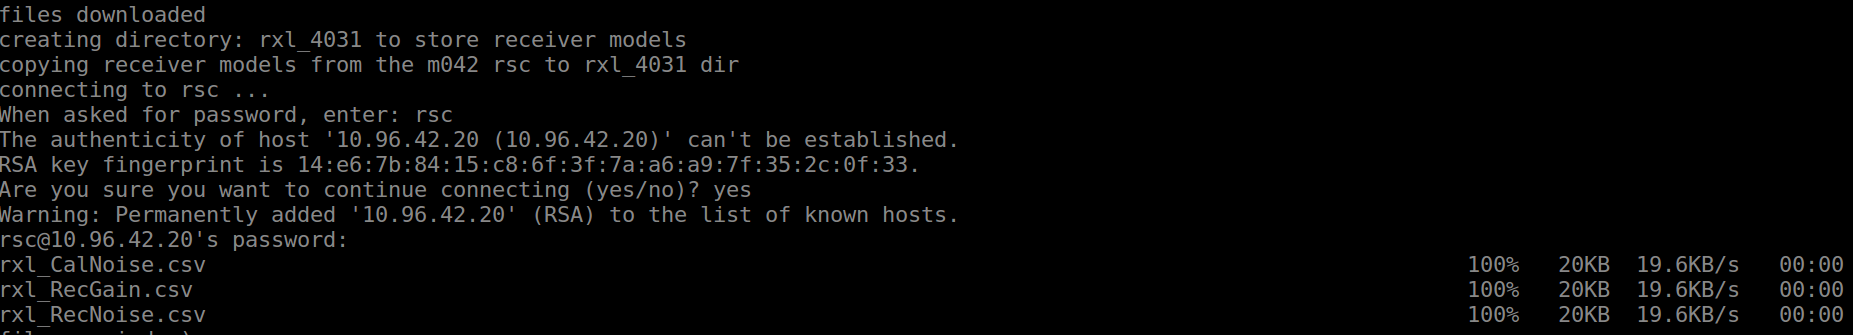
\includegraphics[scale=0.5]{Chapters/images/image25.png}
	
	%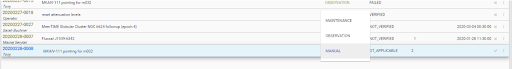
\includegraphics[resolution=100]{bur1.png}
	\caption{Receiver model files downloaded}
	\label{fig:image25}
\end{figure}

\item Later you will be asked a few times to enter your GitHUb credentials (username and password).

\begin{figure}[!thb]
	\centering
	%\includegraphicsdpi{100}{}{bur1.png}     
	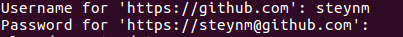
\includegraphics[scale=0.5]{Chapters/images/image14.png}
	
	%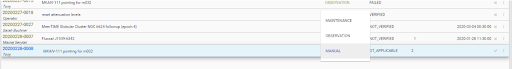
\includegraphics[resolution=100]{bur1.png}
	\caption{Receiver model password}
	\label{fig:image14}
\end{figure}


\item When the script gives the below message then it was successful in uploading files to GitHub and you can proceed to step 3.


\begin{figure}[!thb]
	\centering
	%\includegraphicsdpi{100}{}{bur1.png}     
	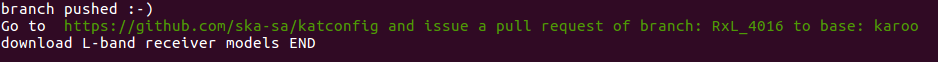
\includegraphics[scale=0.5]{Chapters/images/image80.png}
	
	%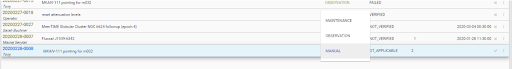
\includegraphics[resolution=100]{bur1.png}
	\caption{Receiver model git push succesful}
	\label{fig:image80}
\end{figure}


\item[\textbf{Step 3}] Issue a pull request on GitHub to merge the branch created in step 2 above to the karoo branch as follows:



\item  Go to \url{https://github.com/ska-sa/katconfig} where you will land at the following page:

\begin{figure}[!thb]
	\centering
	%\includegraphicsdpi{100}{}{bur1.png}     
	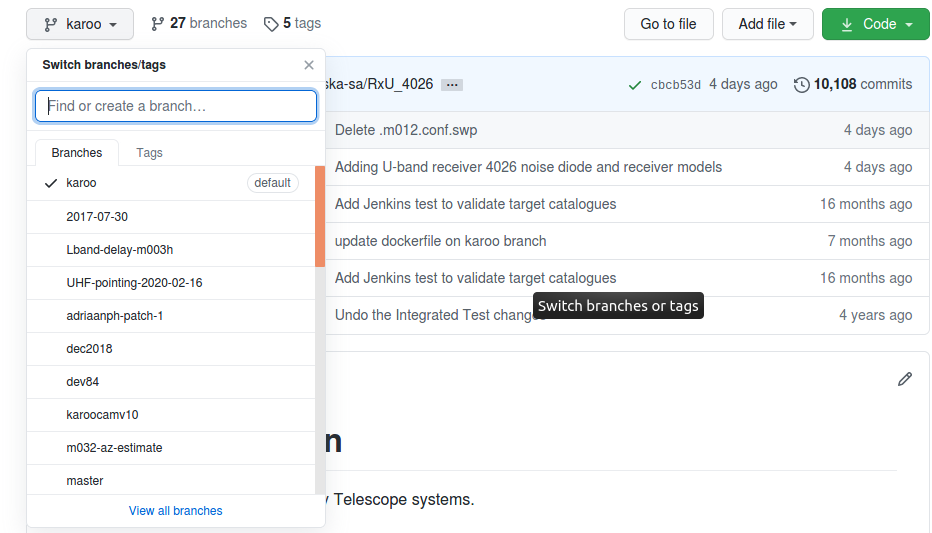
\includegraphics[scale=0.5]{Chapters/images/image108.png}
	
	%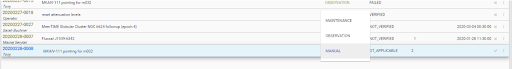
\includegraphics[resolution=100]{bur1.png}
	\caption{Receiver model github compare and pull request}
	\label{fig:image108}
\end{figure}

\item Click on “Compare \& pull request”.
\item Make sure “base: karoo” and “compare: Rx(L or U)\_xxxx” is selected. Then write a comment stating what you are doing, why (give Jira number if applicable) and make the request out to Pieter Kotze. Below is an example:

\begin{figure}[!thb]
	\centering
	%\includegraphicsdpi{100}{}{bur1.png}     
	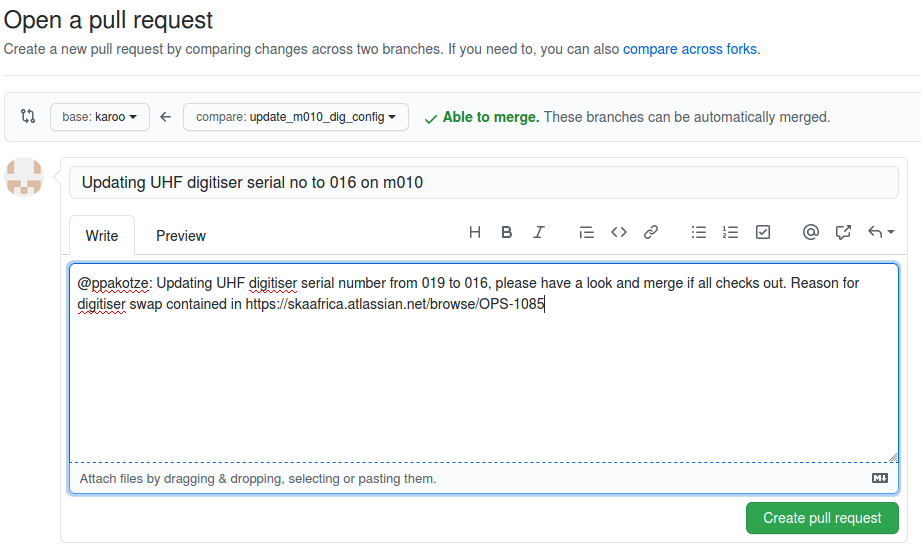
\includegraphics[scale=0.5]{Chapters/images/image81.png}
	
	%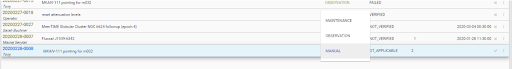
\includegraphics[resolution=100]{bur1.png}
	\caption{Receiver model github pull request}
	\label{fig:image81}
\end{figure}
\item At the right hand side at the top next to “Reviewers”, click on the gear icon. It will drop down a list of reviewers to choose from. Type “ppakotze” in the search field to find Pieter K and then click on Pieter K to request him to approve your pull request (It will show a check mark next to his name, and then under “Reviewers” you will see a yellow dot next to his name).

\begin{figure}[!thb]
	\centering
	%\includegraphicsdpi{100}{}{bur1.png}     
	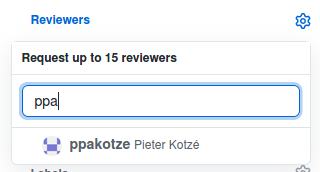
\includegraphics[scale=0.9]{Chapters/images/image57.png}
	
	%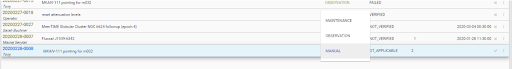
\includegraphics[resolution=100]{bur1.png}
	\caption{Github add pull request reviewers }
	\label{fig:image57}
\end{figure}

\item Then click on “Create pull request”. 
Note: After Pieter K approves the pull request, he usually also merges the pull request, but sometimes you have to do the merging yourself. You do this by going to the pull request after it has been approved, and then click on “Merge pull request” at the bottom and then “Confirm merge”.
\item Proceed to step 4.

\item[\textbf{Step 4}]  Update the table found in this document with the latest value of the “rsc.rx?.rec-model-date” sensor (where ? indicates the band) for the antenna and band whose receiver models were updated.
\end{itemize}


\section{ Checklist after new receiver installation}
\begin{enumerate}
	

\item Check for Ben’s handover from the specific jira
\item Check \sensor{rsc.rxl.startup-state} from sensor list - it should be cold-operational 
\item Check \sensor{rsc.rxl.rfe1.temperature} from sensor list which should around 19 K
\item Check receiver models and compare with those in the katconfig as per procedure above.
\item Run reset attenuations - if power is out of range then proceed to step 6 otherwise proceed to step 7. 
\item Run refine attenuations
\item Run delay calibrations 
\item If the results from delay cal are too high or too low create a jira to Marcel Gouws 
\end{enumerate}

\section{Receiver Vacuum Pump Oil Lubrication}
\textbf{CAUTION}:
\textit{Prevention or little oil available in key receiver areas that need to be lubricated. The lubrication is necessary over a period of 2 weeks. Include as many antennas as possible since CBF and SDP are not required. If the antennas are not  lowered down this could cause serious problems.}
\begin{itemize}


\item  Wait for the flight departure on site. Needs to be above 16 deg C ambient as well (NB for winter)
\item Build a subarray with many free antennas as possible
\item Leave out the receiver band, cbf and sdp
\item Lower the antennas 18 degrees elevation. Use the receptor flight stow script
\item If antennas go into stow or someone moves the antenna to higher elev while the script is busy running, please notify Ben Jordaan about the event.
\item If the script is interrupted before Vacuum pumps are enabled, notify Ben urgently. 
\item Report to Ben which antennas did not start / stop the script.
\item If the Vacuum pump lubrication script does not work / is interrupted on a  certain antenna notify Ben.
\item Run the schedule below to lubricate the receivers
\end{itemize}

\begin{lstlisting}[style=DOS]
configure_obs()
obs.sb.new(owner='MeerKAT')
obs.sb.type = katuilib.ScheduleBlockTypes.OBSERVATION
obs.sb.antenna_spec = 'available'
obs.sb.controlled_resources_spec = ""
obs.sb.description = 'MeerKAT: Lubricate Vacuum Pumps'
obs.sb.instruction_set = "run-obs-script /home/kat/katsdpscripts/utility/lubricate_vacuum_pump.py -n 'off' --proposal-id=VAC_PUMP --program-block-id='RTS Vacuum Pump' "
obs.sb.notes= "projectID=RTS "
obs.sb.to_defined()
obs.sb.to_approved()
\end{lstlisting}


\section{ S-band Operations}

Note: When there is a schedule for S-band testing, Pieter Kotze would usually attend and either do the S-band testing himself, or ask you to build the S-band array and run observations with clear instructions either in the calendar or directly to you on IRC.


The following are most important sensors to check in order to know which antennas are usable for S-band building:
\begin{itemize}
\item The \sensor{rsc\_rxs\_temvac\_temp15K} sensor as shown in \textbf{Figure}~\ref{fig:image48} can be used to determine if S-band receiver is cold.  If the above sensor is under 30\unit{K},  then the receiver is usable.
\begin{figure}[!thb]
	\centering
	%\includegraphicsdpi{100}{}{bur1.png}     
	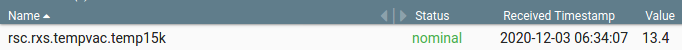
\includegraphics[scale=0.5]{Chapters/images/image48.png}
	
	%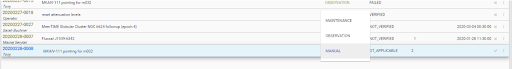
\includegraphics[resolution=100]{bur1.png}
	\caption{S-band receiver temperature sensor}
	\label{fig:image48}
\end{figure}
\item The \sensor{dig.s-band.time.synchronisation-epoch} sensor as shown in \textbf{Figure}~\ref{fig:image85}  can be used to check if the S-band digitiser is synced correctly.
\end{itemize}


\begin{figure}[!thb]
	\centering
	%\includegraphicsdpi{100}{}{bur1.png}     
	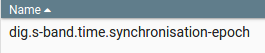
\includegraphics[scale=0.7]{Chapters/images/image85.png}
	
	%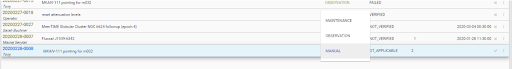
\includegraphics[resolution=100]{bur1.png}
	\caption{S-band time synchronisation epoch sensor}
	\label{fig:image85}
\end{figure}
If the sync epoch is not correct (is not the same number as the others), then an absent/ready cycle is needed on the digitiser for it to receive the right epoch.\\

Note that the conventional commands for marking digitisers absent/ready do not work yet for S-band digitisers, hence you need to use the following commands on obs machine:
\begin{itemize}
	 
\item Make sure the “\sensor{dig-selected-band}” sensor is not currently on ‘s’.
\item To mark the digitiser absent, use
\begin{lstlisting}[style=DOS]
kcpcmd -s 10.103.254.2:72xx digitiser-status s absent
\end{lstlisting}


\item To mark the digitiser ready, use:
\begin{lstlisting}[style=DOS]
kcpcmd -s 10.103.254.2:72xx digitiser-status s ready 
\end{lstlisting}


In the steps above \option{xx} indicates the antenna number. Once the above mentioned sensors are all correct, the antennas should be usable for S-band observations. 

\item Note: A quick way to check the above mentioned sensors is with these commands in an ipython session:
\begin{lstlisting}[style=DOS]
cam.print_sensors('temp15k')
cam.print_sensors('s.band.time.synchronisation.epoch')
\end{lstlisting}
\end{itemize}

\section{ How to build an array}
\textbf{NOTE:} \textit{Only dashes will be displayed next to “NGS” on the GUI when building in S-band. It’s normal for now and does not mean that the S-band digitisers are not synced. As mentioned before, if the epoch of the digitisers are correct, they are synced and ready.}\\

Usually you build an array with:
\begin{itemize}
 

\item  Product = c875M4k (Band = s)
\begin{itemize}
\item[$\circ$]Note: 4k and 32k builds in S-band are normally stable, but only 4A 1k S-band builds work (other 1k S-band builds still have CBF issues).
\end{itemize}
\item  Centre frequency = 3062.5MHz (S4)
\begin{itemize}
\item[$\circ$] Note that SDP only supports these center frequencies for S-band: 2843.75 MHz (S3) and 3062.5 MHz (S4) and must be selected manually on the CAM GUI (does not get chosen by default).
\end{itemize}
\item Dump rate = 1s
\item Add cbf\_1 (CMC1) and sdp\_1 resources if you are on subarray 1. Only use CMC2 if instructed to do so.
\item Usable Antennas: Check the OPS Catalyst notice board for the latest on which antennas can be used in S-band.

\end{itemize}

\begin{figure}[!thb]
	\centering
	%\includegraphicsdpi{100}{}{bur1.png}     
	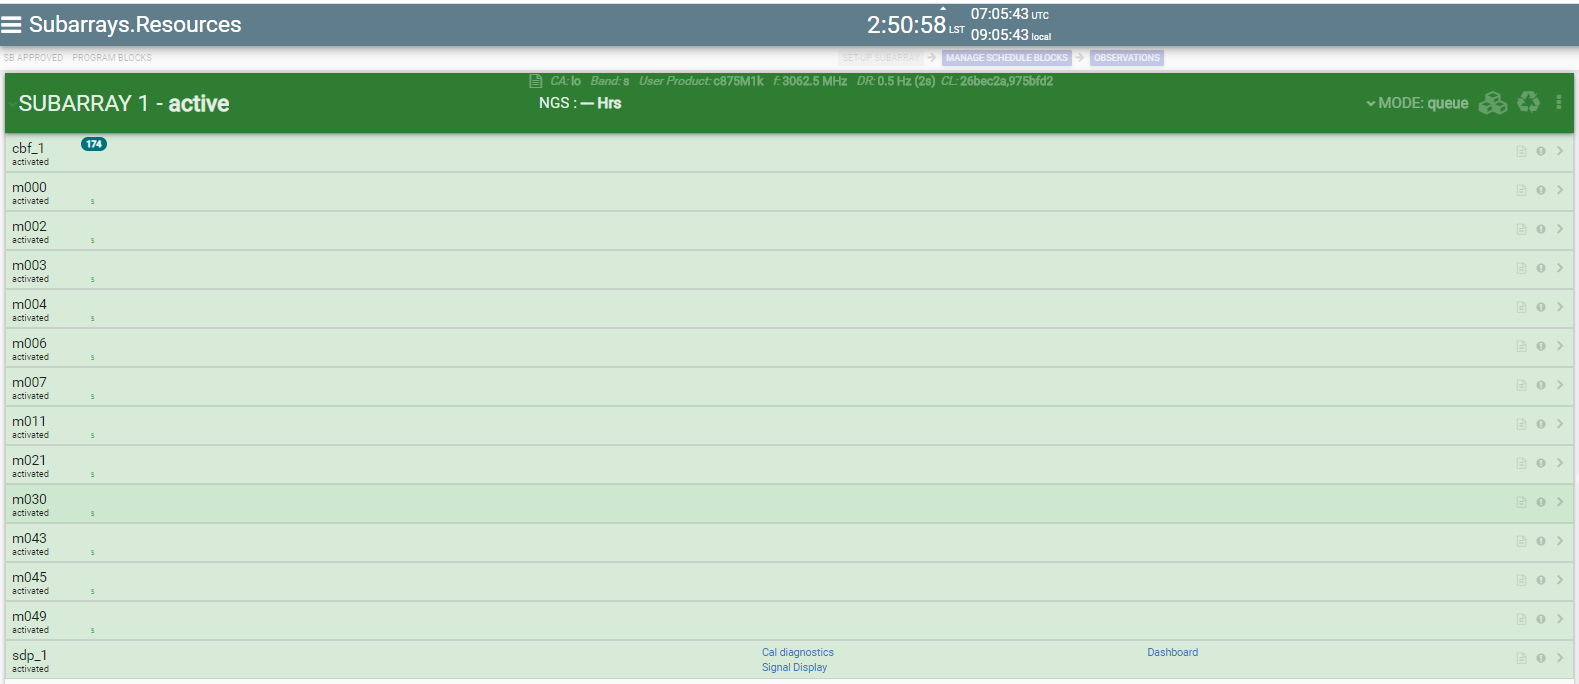
\includegraphics[scale=0.28]{Chapters/images/image113.png}
	
	%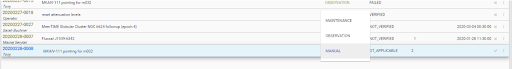
\includegraphics[resolution=100]{bur1.png}
	\caption{Example of a S-band array}
	\label{fig:image113}
\end{figure}



\section{ S-band Observations}
\subsection{ Delay Calibration}
Then run a delaycal:
\begin{itemize}
 \item Example of a good delaycal: \url{http://10.97.1.13:8081/tailtask/20200929-0021/progress }
 \begin{itemize}
\item[$\circ$] Note: \component{M056} vpol has an unstable signal power (visible on the timeseries), however you still include AP in S-band observations (\textbf{don’t mark it faulty}).
\end{itemize}
If you see strangeness on antennas not AP failure related (saturation, weird power levels, noisiness, large delay offsets, no delay solutions etc), keep them in (don’t mark them faulty) for Single dish RTS observations (phase stability, drift scans, tipping curve etc.) as RTS still wants their data. Can only exclude the APs for observations such as S-band holography.
\end{itemize}
\subsection{ Example of schedule blocks}
Description:
\begin{lstlisting}[style=DOS]
obs.sb.new(owner='RTS')
obs.sb.type = katuilib.ScheduleBlockTypes.OBSERVATION
obs.sb.description = 'RTS: S-band Drift Scan of Hyd A'
obs.sb.antenna_spec = 'available'
obs.sb.controlled_resources_spec="cbf, sdp"
obs.sb.proposal_id = 'COMM-RTS'
obs.sb.instruction_set= "run-obs-script /home/kat/usersnfs/benjamin/drift_scan_2.py 'hyda' --drift-duration 1800 "
obs.sb.notes= "reductionid='N/A' , projectID=RTS "
obs.sb.to_defined()
obs.sb.to_approved()
\end{lstlisting}


\subsection{ Phase stability} 
While you have S-band built phase stability could also be run on Hydra A.
Just remember it will need a delay\_Cal.
\begin{lstlisting}[style=DOS]
obs.sb.new(owner='RTS')
obs.sb.type = katuilib.ScheduleBlockTypes.OBSERVATION
obs.sb.description = 'RTS: 3.1.2.1 S-band Interferometric Phase Stability hyda '
obs.sb.antenna_spec = 'available'
obs.sb.controlled_resources_spec="cbf, sdp"
obs.sb.proposal_id = 'COMM-RTS'
obs.sb.instruction_set= "run-obs-script /home/kat/katsdpscripts/RTS/2.9-RFI/track.py 'hyda' --repeat -t 7200 -n 'off' -m 7200 "
obs.sb.to_defined()
obs.sb.to_approved()

\end{lstlisting}

\subsection{ Tipping curve }
Additionally a tipping curve could be useful.
Same array configuration, can be run anytime during the day or night and takes about 1.5 hours.
\begin{lstlisting}[style=DOS]
obs.sb.new(owner='RTS')
obs.sb.type = katuilib.ScheduleBlockTypes.OBSERVATION
obs.sb.description = 'RTS: 2.1 S-band Tipping_Curve'
obs.sb.antenna_spec = 'available'
obs.sb.controlled_resources_spec="cbf, sdp"
obs.sb.proposal_id = 'COMM-RTS'
obs.sb.instruction_set= "run-obs-script /home/kat/katsdpscripts/RTS/2.1-Tipping_Curve/obs_tipping_curve.py  "
obs.sb.notes= "reductionid='2.1' , projectID=RTS "
obs.sb.to_defined()
obs.sb.to_approved() 

\end{lstlisting}


